\documentclass[11pt, oneside]{article} 
\usepackage{geometry}
\geometry{letterpaper} 
\usepackage{graphicx}
	
\usepackage{amssymb}
\usepackage{amsmath}
\usepackage{parskip}
\usepackage{color}
\usepackage{hyperref}

\graphicspath{{/Users/telliott/Github/calculus_book/png/}}
% \begin{center} 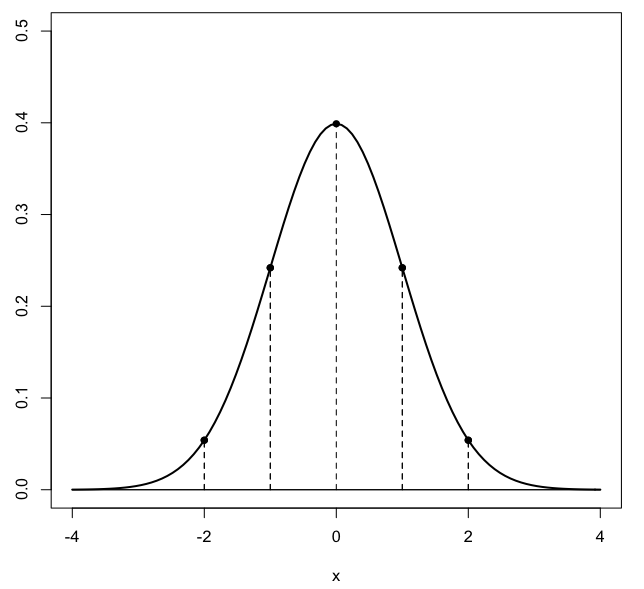
\includegraphics [scale=0.4] {gauss3.png} \end{center}

\title{Induction}
\date{}

\begin{document}
\maketitle
\Large

\label{sec:Induction}

We can visualize an inductive proof as a kind of chain.  We show that the "base case" is true, for some value of $n$.  Then we show that if the formula works for $n$ , it must work for $n+1$.

\begin{quote}Mathematical induction proves that we can climb as high as we like on a ladder, by proving that we can climb onto the bottom rung (the basis) and that from each rung we can climb up to the next one (the step).\end{quote}

- Graham, Knuth and Patashnik

[ There is a variant called \emph{strong} induction where we assume some statement is true for \emph{all} $0 < k \le n$. ]

\subsection*{the problem}

Suppose we have some theorem that we \emph{think} might apply to all $k \le n$.  A classic example (Courant and Robbins?) is:
\[ f(n) = n^2 - n + 41 \]
The function $f(n)$ produces a prime number for $n \in [1..40]$, which is apparent by inspection (because $41$ is prime).  But for $n=41$ all terms are divisible by $41$, thus the result cannot be prime.

Hamming has some other examples.  Here is one:
\[ f(n) = n(n-1)(n-2) \dots (n-k) \]
$f(n)=0$ for all $0 \le n \le k$, but will never be zero for any other $n > k$!  By choosing $k$ large, we can make the number of true cases as large as you like.

Furthermore, for any function $g(n)$, $f(n) + g(n)$ will have the same property.

\subsection*{proof of induction}

According to Hamming, if you are not convinced by the ladder analogy, here is another proof that induction works:

\begin{quote}Suppose the statement is not true for every positive (non-negative) integer.  Then there are some false cases.  Consider the set for which the statement is false.  \emph{If} this is a non-empty set, then it would have a least integer, which is $m$.  Now consider the preceeding case, which is $m - 1$.  This $(m-1)$th case must be true by definition, and we know that there is such a case because as a basis for the induction we showed that there was at least one true case.  We now apply the step forward, starting from this true case $m-1$, and conclude that the next case, case $m$, must be true.  But we assumed that it was \emph{false}!  A contradiction. \end{quote}

Therefore, there are no false cases.

\subsection*{sums of integers}

Later in the book, we will compute Riemann sums, and to do that we need to find formulas for the sum of integers, the sum of square integers, and so on.  

To keep it simple, let's start with finite sums like the integers from $1$ to $n$
\[  1 + 2 + 3 + \cdots + n  \]
The numbers we seek are called the triangular numbers.  These are
\[ 1, 3, 6, 10, 15 \cdots \]
Here is a striking "visual proof" of the formula to obtain T$_n$, the $n^{th}$ such number.  The total number of circles in the figure below is $n \times (n+1)$ and this is exactly two times the sum of the integers from $1$ to $n$.

\begin{center} 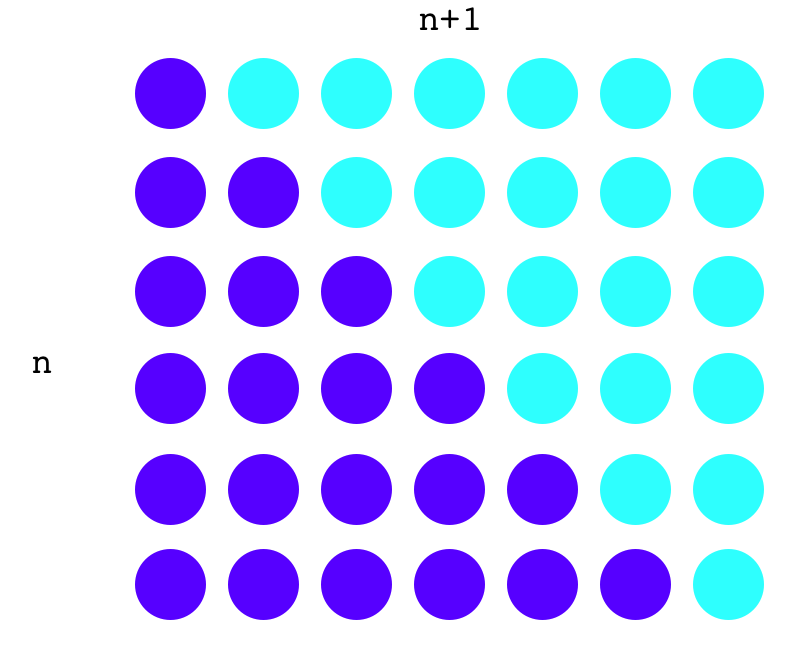
\includegraphics [scale=0.25] {sum_n.png}\end{center}
\[ 2S = n(n+1) \]
There is a famous story about Gauss that, as a schoolboy, he "saw" how to add the integers from $1$ to $100$ as two parallel sums
\[ \ \  1 + \ \ 2 + \ \ 3 + \cdots + 99 + 100 \]
\[ 100 + 99 + 98 + \cdots + 2 + 1 \]
Added together horizontally, these two series must equal twice the sum of $1$ to $100$.  But in the vertical, we notice that we have $n$ sums, each of which is equal to $n+1$.  So, again
\[ 2S = n (n+1) \]
\[ S = \frac{1}{2} \ n (n+1) \]
For $n=100$ the value of the sum is $5050$.  Another way of looking at this result is that between $1$ and $100$ there are $100$ representatives of the "average" value in the sequence, which (because of the monotonic steps) is $(100 + 1)/2 = 50.5$.  

Or alternatively, view the sum as ranging from $0$ to $100$ (with the same answer).  Now there are $101$ examples of the average value ($100 + 0)/2 = 50$).

\subsection*{Proof of the formula $n(n+1)/2$ by induction}

Returning to the sum of integers, one proof follows the method of induction.  In this approach, however, one must first guess the correct formula.  We guess $n(n+1)/2$, of course.

For this example of induction, we will assume the formula is true for $n-1$ and show that if so, it is true for $n$.  Hamming says this may be easier sometimes than starting with $n$.

So, we \emph{assume} that the answer is correct for $n - 1$.  In this case, the formula changes to
\[ S_{n-1} = \frac{n(n-1)}{2} \]
So clearly, if $S_{n-1}$ is correct, then
\[ S_{n} = S_{n-1} + n \]

Follow out the arithmetic:
\[ = \frac{n(n-1)}{2} + n \]
\[ = \frac{n(n-1) + 2n}{2} \]
\[ = \frac{(n^2 + n)}{2} \]
\[ = \frac{n(n+1)}{2} \]

But this is precisely what we would obtain by using the formula, and substituting $n$ for $n - 1$.  Hence the formula gives the correct result for $n$, assuming that it gives the correct result for $n-1$. 

In turn, it gives the correct result for $n-1$, assuming it gives the correct result for $n-2$.  Eventually, we reach the base case, where we can verify that the result is correct.

Try it on the first value in the sequence ($n=1$, the "base case").
\[ \frac{1(0)}{2} = 0 \]
That checks. If you're worried check $n=2$:
\[ \frac{2(1)}{2} = 1 \]

So the whole chain of reasoning is correct.  

$\square$

\subsection*{geometric example}

In the figure below we have a polygon---an irregular heptagon.  Actually, there are three polygons altogether, there is the heptagon with $n+1$ sides, the hexagon with only $n$ sides that would result from cutting along the dotted line, and the triangle that is cut off.

What we would like to do is to find a formula for the sum of the internal angles that depends only on the number of sides or vertices.

\begin{center} 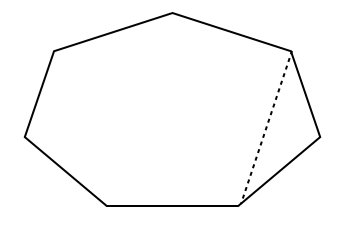
\includegraphics [scale=0.5] {polygon.png} \end{center}

The first part of the answer is to guess.  In the figure, you can see that by adding the extra vertex to go to the $n+1$-gon, we added a triangle, or perhaps you'd rather say than in going from $n+1$ to $n$ we lost a triangle.  

In either case, the difference is $180^\circ$.  The difference between having $n$ sides and $n+1$ sides is to add $180^\circ$.  

The second part of the argument is to suppose that $n=3$, in that case we must have simply $180^\circ$ degrees for a triangle.  So we guess that the formula may be
\[ (n-2)180^\circ = S_n \]
where S is the sum of the angles in an $n$-gon.

We can use induction to prove that this formula is correct.

The proof has two parts.  We must verify the formula for a base case like the triangle, which we've done.  You may wish to check that it works for the square as well, but that's not strictly necessary.

The second part of the proof is to verify that in going from $n$ to $n+1$, we add another $180^\circ$.  \[ (n-2)180^\circ + 180^\circ \stackrel{?}{=} ((n+1)-2)180^\circ \]
On the left-hand side, we have the sum of angles for $n$ sides, which we assume is correct, and then we just add $180^\circ$ to it.  On the right, we have substituted $n+1$ into the formula.

Now we need to show that these are equivalent.  But of course
\[ (n-2)x + x = ((n+1)-2) x \]
\[ n - 2 + 1 = n + 1 - 2 \]
$\square$

That is the inductive proof of the formula.

\subsection*{sum of integer squares}
\begin{center} 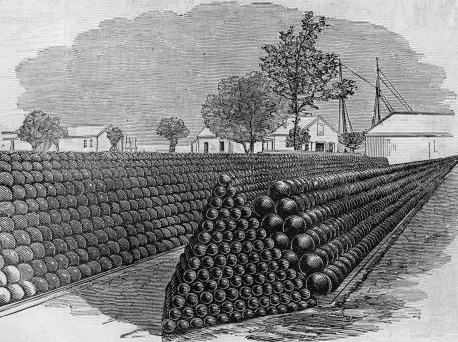
\includegraphics [scale=0.4] {cannonballs.png} \end{center}

Have you ever seen a square stack of marbles, or cannonballs?  The number of elements on each level is the square of a natural number.  We ask, what is the total number:
\[ S = 1^2 + 2^2 + \dots + n^2 = \ ? \]

The answer is not obvious, but we will see how to prove it later using a method called induction.  We will also see how to deduce it.  For now it is enough to give the result:
\[ S = \frac{1}{3} \cdot n \cdot (n + \frac{1}{2}) \cdot (n + 1) \]
which is sometimes given as
\[ S = \frac{n(n+1)(2n+1)}{6} \]

Given the formula for the volume of a cone or pyramid, the factor $1/3$ is not surprising.


\end{document}  